%\documentclass[a4paper,10pt,draft,oneside,openbib,openright]{report}
\documentclass[a4paper,10pt,oneside,openright,openbib]{report}

\usepackage[utf8]{inputenc}
\usepackage[american]{babel}
\usepackage[T1]{fontenc}
%\usepackage[dvips,pdftex]{graphicx}
% only for DRAFT purposes
\usepackage[dvips]{graphicx}
\usepackage{makeidx}
\usepackage{pst-all}
\usepackage{subfigure}

\usepackage{ulem}

\usepackage{lastpage}
\usepackage{verbatim}
\usepackage{multirow}
\usepackage{tikz}
\usepackage{wrapfig}
\usepackage[nonumberlist, toc, section]{glossaries}
\usepackage{listings}
\usepackage{multicol}

\usepackage[light]{draftcopy}
%\usepackage[dvips,pdftex]{hyperref}
%
\usepackage{hyperref}
\hypersetup{colorlinks, 
	   citecolor=black,
	   filecolor=black,
	   linkcolor=black,
	   urlcolor=black,
	   bookmarksopen=true,
%	   pdftex}
}


\author{
%Armin Bauer <abauer@>\\ % TODO: ask for permission
Daniel Gollub <dgollub@suse.de>\\
}

\title{\huge{OpenSync}\\\large{A Synchronization Framework}}

\date{\today}


\begin{document}


\maketitle

\begin{quote}
Copyright \copyright{}  2008  Daniel Gollub.
Permission is granted to copy, distribute and/or modify this document
under the terms of the GNU Free Documentation License, Version 1.2
or any later version published by the Free Software Foundation;
with no Invariant Sections, no Front-Cover Texts, and no Back-Cover Texts.
A copy of the license is included in the section entitled ``GNU
Free Documentation License''. 
\end{quote}

\vfill
\begin{center}
(This page is \textbf{not} kept intentionally blank.)
\end{center}
\vfill

\tableofcontents

\newpage

%Abstract
\chapter*{Abstract}
\addcontentsline{toc}{subsection}{Abstract}
This document is a very detailed and technical paper about the OpenSync 
Framework, which gives a brief introduction about what the powerful OpenSync 
Framework provides and could be used for. It also covers lots of internal 
information for (ongoing) OpenSync developers. As well as for OpenSync Plugin 
and/or Frontend authors.\\
\\
Enjoy \& Don't forget to have fun!


%Introduction
\chapter{Introduction}
\label{chap:intro}
OpenSync is intended to be an universal Synchronization Framework, not limited to
a platform or desktop nor to PIM!

\section{History}
MultiSync, started by Bo Lincoln, was intended to synchronize various mobiles,
PDAs and PIM applications. MultiSync was a GTK application and provided
support for different PIM applications and devices by providing  plugins.
Primary focus of MultiSync was to synchronize just PIM data (contacts, 
appointments, notes). Unfortunately this approach was fixed to a single UI and 
only limited to PIM synchronization. Development branch MultiSync 0.9x was 
intended fix those needs.\\
\\
Early in 2005, Armin Bauer started refactoring the MultiSync project and
separated the UI code from MultiSync and the Plugin interface and
Synchronization logic. Result of his work is the most powerful and
flexible Synchronization Framework, known today as OpenSync.
\section{Big Picture}
OpenSync is intended to provide a low-level synchronization API for all kind of 
data.
\\
\begin{figure}
 \centering
 % \includegraphics[bb=0 0 222 140,scale=0.5]{bigpicture}
 % bigpicture.png: 222x140 pixel, 72dpi, 7.83x4.94 cm, bb=0 0 222 140
 \caption{OpenSync}
 \label{fig:bigpicture}
\end{figure}


\section{Goals}
The goals of the OpenSync project are:

\begin{itemize}
 \item Reusabilty. OpenSync should be usable for all kind of synchronization 
 applications
 \item Speed. Synchronization should be efficent and fast as possible to give the
 user the best experience.
 \item Flexibility. Nobody can predict what comes next to synchronize; after the
 G- \& iPhone. So OpenSync has to be designed and built as flexible and modular 
 as possible.
 \item Integrity. Data MUST never be lost or malformed, no matter what happens. 
 Data loss is just a no go!
 \item Portability. OpenSync should just run on as many platforms as possible as 
 possible.
 \item Fun. The experience of using and developing OpenSync MUST be fun! You 
 should not work on OpenSync if you're unhappy :)
\end{itemize}
Not all of the mentioned goals are reached already, but OpenSync tries to get 
close as possible over time.

\section{Who should read this document?}
This Document is intended for everyone who is interested in a Open Source 
Synchronization solution. This is not a HowTo, Tutorial or Guide how to use 
OpenSync. It's a detailed introducation in the OpenSync framework. No (high) 
programming skills/experince are required for this document.

\section{How should this document be read?}
Some chapter are very detailed about internal technial stuff, which is mainly 
intended for developers or people who are interested in how OpenSync ticks. Those
chapters could be safetly skipped if someone isn't interested in touching the
internals of the OpenSync Framework. Such section are marked with a little hint.

\section{Is this the most recent version of this paper?}
Maybe not, OpenSync is in a very early stage of development and lots of stuff
might changed within the last weeks. On doubts you might compare your version 
with the one from:\\
\\
\hyperref[http://www.opensync.org/download/LATEST-WHITEPAPER]{http://www.opensync.org/download/LATEST-WHITEPAPER}\\
\\
This paper was created on: \today


%Synchronization
\chapter{Synchronization}
This chapter give a brief introduction of synchronization basics as well as how
OpenSync works and handles real life synchronization issues.\\
\\
Different synchronization techniques used nowadays, which have some of the
following tasks in common:
\begin{itemize}
 \item Connect
 \item Get changes
 \item Conflict resolution
 \item Multiply changes
 \item Commit changes
 \item Disconnect
\end{itemize}
Those tasks are in common for synchronization technique/protocol, but differ in
detail to fit the needs for different circumstances to meet the best efficiency.
Such circumstances could be:
\begin{itemize}
 \item Number of synchronization parties. If the number of synchronization
 parties is two, then multiplying of changes is just simple duplication of the
 change.
 \item Unidirectional/Bidirectional synchronization. On unidirectional
 synchronization no conflict resolution required for two parties.
 \item Resource. Depending of the type of data resource further work is required
 to get changes. Is the resource able to tell which data changed since the last
 synchronization, by its own? Or is further help/facility required to detect
 which data changed since the last sync. Example: file systems, databases,
 stacked data in a single file, ...
 \item Type of data. Is the data in a consistent format and supported by all
 parties? File synchronization. Is the data not consistent and contains unique
 information which doesn't allow to do a binary compare? Weak compare? Is 
 conversion to a common format for different parties required?
 \item Protocol. Does the protocol require to read only the latest changes or 
 all at once? Does the protocol support single commits or only all at once 
 (batch commit)?
 \item Transport. Are various transport layer involved? Does it require to
 connect and disconnect in a specified way? Limited bandwidth? Example: 
 Bluetooth, USB, ...
\end{itemize}
You see, there lots of different circumstances which makes it quite complicated
to meet all the needs of different ways to synchronize and synchronization 
protocols.\\
This is also only the tip of the iceberg, since it describes only the
synchronization role of the ">Server"<. 

\section{Synchronization Role}
The term ">Server"< is quite confusing,
especially in the combination of a synchronization protocol which uses a
transport protocol based on the ">Client"<- and ">Server<"-Model. Most famous
example is ">SyncML"<, which support among others the HTTP and OBEX protocol as
transport. You might know ">HTTP Server"< like the Apache Webserver and ">HTTP
Client"< like the Firefox Webbrowser. In SyncML you can have for example (same 
for other transports supported by SyncML):
\begin{itemize}
\item HTTP Server transport and act as Synchronization Server
\item HTTP Client transport and act as Synchronization Server
\item HTTP Server transport and act as Synchronization Client
\item HTTP Client transport and act as Synchronization Client
\end{itemize}
OpenSync doesn't care much about Transport Server/Client role, this is
up to the Plugins. There is only a little detail which OpenSync have to care
about plugin when they're acting as the transport Server role, which is about
that the plugin has to be initialized all the time so the client can connect.
More about this in the Plugin chapter.\\
\\
Unfortunately OpenSync supports in version 0.40 only the Synchronization role
Server. The passive role as Synchronization Client isn't yet implemented, but is
on the top of the project agenda. The reason for this is that the current
implementation of synchronization tasks/steps mentioned above are currently
fixed. As Synchronization Client the order and number of this synchronization 
steps/tasks would differ to the Server role. More about this issue you can find
in the Framework Chapter in section Synchronization Role.

\section{Slow Sync}
Various Synchronization protocols are using so called ">Slow Sync"<
synchronization technique. This consists of two types of synchronizations, the
already mentioned ">Slow Sync"< and a regular Synchronization (sometimes called
">Fast Sync<"). The difference between the Slow and the regular (Fast) Sync is 
that the regular one only transfers changes since the last synchronization. 
This means on a regular synchronization not all entries have to be transfered, 
converted. This makes the synchronization quite efficient and very fast. The
so called ">Slow Sync"< requests intentionally all entries, which makes the
synchronization a bit slower. Additionally the Synchronization Framework has to
interpret every single entry/change as newly added, since the Framework vanished
in advance the entire mappings and has to compare every single reported entry
from each party and find the fitting counterpart. This and the combination of
transferring all entries makes the synchronization compared to the regular
(Fast) synchronization very slow. The ">Slow Sync"< is only used in certain
cases to avoid data inconsistence and to keep all the data in sync. ">Slow
Sync"< got emitted in following circumstances:
\begin{itemize}
\item First/Initial Synchronization
\item Party got reseted (same as first sync)
\item Party got synchronized in meanwhile within another environment 
\item After an aborted/failed synchronization
\end{itemize}
\section{Object Types}
The term ">Object Types"< is in OpenSync used to describe the type/category of 
data. Example for ">Object Types"< are Contacts, Events, Todos, Notes or plain 
Data (like the content of a file) and others. (It's not limited to PIM Data!). 
Those Object Types get separated processed, to make it configurable which 
Object Type should get synchronized. Example: Only synchronize contacts of the 
mobile, no events, todos nor notes.
\section{Formats}
The ability to synchronize different Parties which use different formats, makes
the OpenSync Framework to a very powerful Synchronization Framework. In OpenSync
each Format is associated with one Object Type (see previous chapter). This
Object Type as common denominator for different formats makes it possible to
determine a conversion path between different formats. The conversion path
consists of various format converters, which are provided by Format Plugins.
Example: Two parties should synchronize their contacts (the Object Type). Party
A stores the contacts as VCard 3.0 and Party B stores the contacts in some
Binary Format. To synchronize the VCard 3.0 and the Random Binary Contact Format
format plugins have to register those formats and provide converters. The
Plugins don't have to provide converters for every known Format, often a certain
amount of converters to common formats or a common denominator format is enough
to create a conversion path between VCard 3.0 to Binary Contact Format.
\section{Mappings}
If an entry got changed on one Party, the logical same entry has to be updated
on the other parties while synchronization. Often different parties use
different ids to identify their entries. So it's required to map the logical
same entries which each others native id. The combination of those different
entries on different parties are called ">Mappings"<. Those ">Mappings"< make it
possible to determine a conflict if mapped entries got changed on different
parties the same time in a different way.
\section{Conflicts}
So called ">Conflicts"< appear if at least two entries of the same mapping got
changed in a different way. No conflict appears if all entries of the mapping
changed the same way. Such conflicts have to be handled by the Synchronization
Framework to avoid data loss. There are several ways to solve such conflicts.
OpenSync provides several different for a proper conflict resolution without
gaining unintended loss of data. Following conflict resolution are supported by
the OpenSync Framework:

\begin{itemize}
\item Solve, means intentionally choosing one of the conflicting entries to
solve the conflict. The chosen one will be multiplied to all parties and will
overwrite the other conflicting changes. This also allows to configure in
advance who is the ">Winning"< Party, who's changes will always used as the 
solving change (">master change"<) for the conflict.
\item Duplicate, (intentionally) will duplicate all changed entries. 
\item Latest, using the latest changed entry of the conflicting entries. This is
only an conflict resolution option if all changes provide within their formats
enough information to determine which got most recently changed.
\item Ignoring, (temporarily) the conflict till the next synchronization.
Conflicting entries will be read and compared again by the OpenSync Framework on
the next synchronization. To avoid inconsistence and data loss. If the
entries/changes are equal on the next synchronization the conflict is solved as
well. (This conflict resolution requires that the protocol of all parties is
able to request single entries, without triggering a "Slow Sync".)
\end{itemize}
\section{Capabilities}
\section{Filter}
OpenSync provides initial code for filtering, but it's not yet usable within
OpenSync 0.40. Looking forward to OpenSync 0.41!


%Framework Architecture
\chapter{Framework Architecture}

\section{IPC}
Part of the OpenSync framework is an Interprocess Communication system to
communicate with the Plugins. To avoid confusion between the different process
types of Plugins, and to make the IPC independent of Plugins, the neutral terms
">Client"< and >"Client Proxy<" got introduced. The IPC is allows full duplex 
(bidirectional) communication between Client and Proxy. Independent of the 
process type of the Client. The frameworks allows to communicate between three 
different process types of Clients:
\begin{itemize}
\item Threaded via pipes (two pipes for full duplex/bidirectional ipc. See
pipe(7))
\item Forked via pipes (two pipes for full duplex/bidirectional ipc. See pipe(7))
\item External process via named pipes (FIFO)
\end{itemize}
This IPC also to send specific type of messages between the Client and the
Proxy. The Proxy takes care about timeout handling, if a client doesn't
response in time. This is only supported for messages which have a callback
function assigned. Such callbacks (command handler) get executed as soon if the
message reply by the Client is retrieved. On a timeout or error the callback
function got called with the custom error or timeout message.

\subsection{Client}
Clients handle all requests from the Proxy. Each request from the proxy gets
replied. Threaded and Forked clients get started by the Proxy. Most common use of
the Client is to call Plugin specific functions, requested with message send by
the Proxy. The client replies the result of the function calls with replying to
the messaged which requested the event.

\subsection{Proxy}
The Proxy handles all request to and from the Client. For each Client there is
one Proxy. The proxy got mainly used by the OpenSync framework engines to
communicate with the Plugin processes.

\subsection{Messaging Queues}
The communication between Client and Proxy is based on message queues. There are
two types of such Queues: Sender- and Receiver-Queue. The Queue object supports
(anonymous) pipes as well as named pipes (FIFO).\\
\\
Note: When using Queues along forked processes the read and write ends have to
be disconnected/closed for proper communication. See pipe(7).\\
\\
There is a specified set of Message Commands for simple communication between
Client and Proxy. For synchronized communication between Client and Proxy the
Client simply replies the Message Command from the Proxy, when Client executed
the requested command. If Client failed while executing the command, it has to
reply with an error reply. Synchronize communication requires that the caller
assign a message handler to the Message object, which got called when the
message got replied. This message handler should check carefully the received
replied message type, and handle provide proper error handling.\\
\\
For synchronized communication it's recommended to send message with a timeout
via the message queue. To avoid deadlocks when the counterpart fails to reply.
No timeout handling is needed for asynchronized communication without command
handler, since no reply is expected.\\
\\
Additional content of the message have to be marshaled/demarshaled, to make the
content usable even it's running in a different address space. (rough rule of 
thumb: everything which includes a pointers/memory addresses)

\section{Engines}
So called engines are the core of the entire framework and control the entire
sequence of every single step which is done during a synchronization. When the
engine got initialized it checks if a previous synchronization was unclean
(failed) and a slow sync is required. If the previous synchronization was
unclean or not could be only determined by engine itself if an group environment
is used. Beside the group environment it also initializes the plugin, format.
The engine isn't restricted to get called with a group environment, the group 
environment is only of optional use.\\
\\
If the group environment is used, the engine locks the group when the engine
gets initialized. If the group detects an unassigned lock the engine will
request while synchronization a slow sync.\\
\\
To determine a previous unclean synchronization without a group environment , 
it's up to OpenSync framework using program to provide facilities to store such 
information. If so, the engine MUST be set to trigger a slow sync, after it got 
initialized. When the engine got finalized or synchronized successful the slow 
sync engine status got reseted.\\
\\
With the engine initialization also the members of the group got initialized.
The member initialization creates for corresponding member plugin a Client Proxy
which got initialized and spawns the plugin. For more details check the IPC
section about the Proxy.\\
\\
After all members got initialized, the >"Object Engines<" for each enabled
Object Type got initialized. If no Object Type is enabled or discovered the
engine initialization aborts with an error. The engine needs at least one Object
Type to synchronize. Often this error appears if not all or none members got
discovered. See discover section of "Merging capabilities" for more details.

\subsection{Object Engine}
For each Object Type, which have to be synchronized, one Object Engine gets 
started by the (main) engine. If the engine detected that previous 
synchronization was unclean, each Object Engine get the slow sync flag set to 
perform a slow sync on the next sync. If the Object Engine got finalized or 
synchronized (successful or unsuccessful) the slow sync flag get reseted. If 
the synchronization failed, it's most likely that the (main) engine will set 
the slow sync flag again on the next synchronization.\\
\\
The Object Engines allows to perform actions only for a certain Object Type. For
example to request a slow sync only for specific Object Engines (this means also
for specific Object Types).\\
\\
The initialization of an Object Engine creates for each Client Proxy (read 
Members' Plugin) a Sink Engine, which maps each Client Proxy with an Object
Type. (More about the Sink Engine in the next section.)\\
\\
If a slow sync got set for the Object Engine, then all >"Mappings<" with the
Object Type of the Object Engine got deleted from the >"Mapping Table<". This is
done to avoid loss of the data inconsistence while performing a slow sync.\\
\\
If no slow sync got set for this Object Engine the >"Mapping Table<" got loaded
and creates for each Mapping a >"Mapping Engine<".

%TODO: Injecting ignored entries in mapping engine

%TODO


\subsection{Mapping Engine}
\subsection{Mapping Entry Engine}


\subsection{Sink Engine}
The Sink Engine currently doesn't consists of any logic. The only relation to
Engines of the Sink Engine object is, it maps all the already mentioned engines
together.\\
\\
The Sink Engine maps the Client Proxy and Object Engine together. With this 
combination the Sink Engine is able to handle Object Type specific (aka. 
ObjTypeSink) tasks. Additionally it contains of a list of Mapping Engines, 
which handle Object Type and Client related Mappings only.

\section{Merging Different Capabilities}
\subsection{Capabilities}
\subsection{Archive}
\subsection{Merger \& Demerger}
\section{Helpers}
\subsection{Anchor Table}
\subsection{Hash Table}
\subsection{Time Helper}
\section{Filter}
\subsection{Custom Fiter}


%Plugins
\chapter{Synchronization Plugins}
Synchronization Plugins are modules which provides access to a certain device,
application or protocol. All of those plugins provide independent of the
synchronized content/format or connection type, the same functions:
\begin{itemize}
\item initialize. This function parse the plugin configuration and initializes
the plugin. If the plugin acts as server, it also initializes this one and 
listen for incoming connections.
\item finalize. This function releases all gained memory by the plugin and stops
the listening server if present. 
\item discover. This function is intended to get called initially to gain
information about the target application, device or system. In detail it detects
all supported formats and individual capabilities of this format, if possible.
And basic information about the target application/device like version, vendor,
product, etc. ...
%\item usable. This function is intended to check if the target
%application/device is usable.
\end{itemize}

\begin{figure}
 \centering
 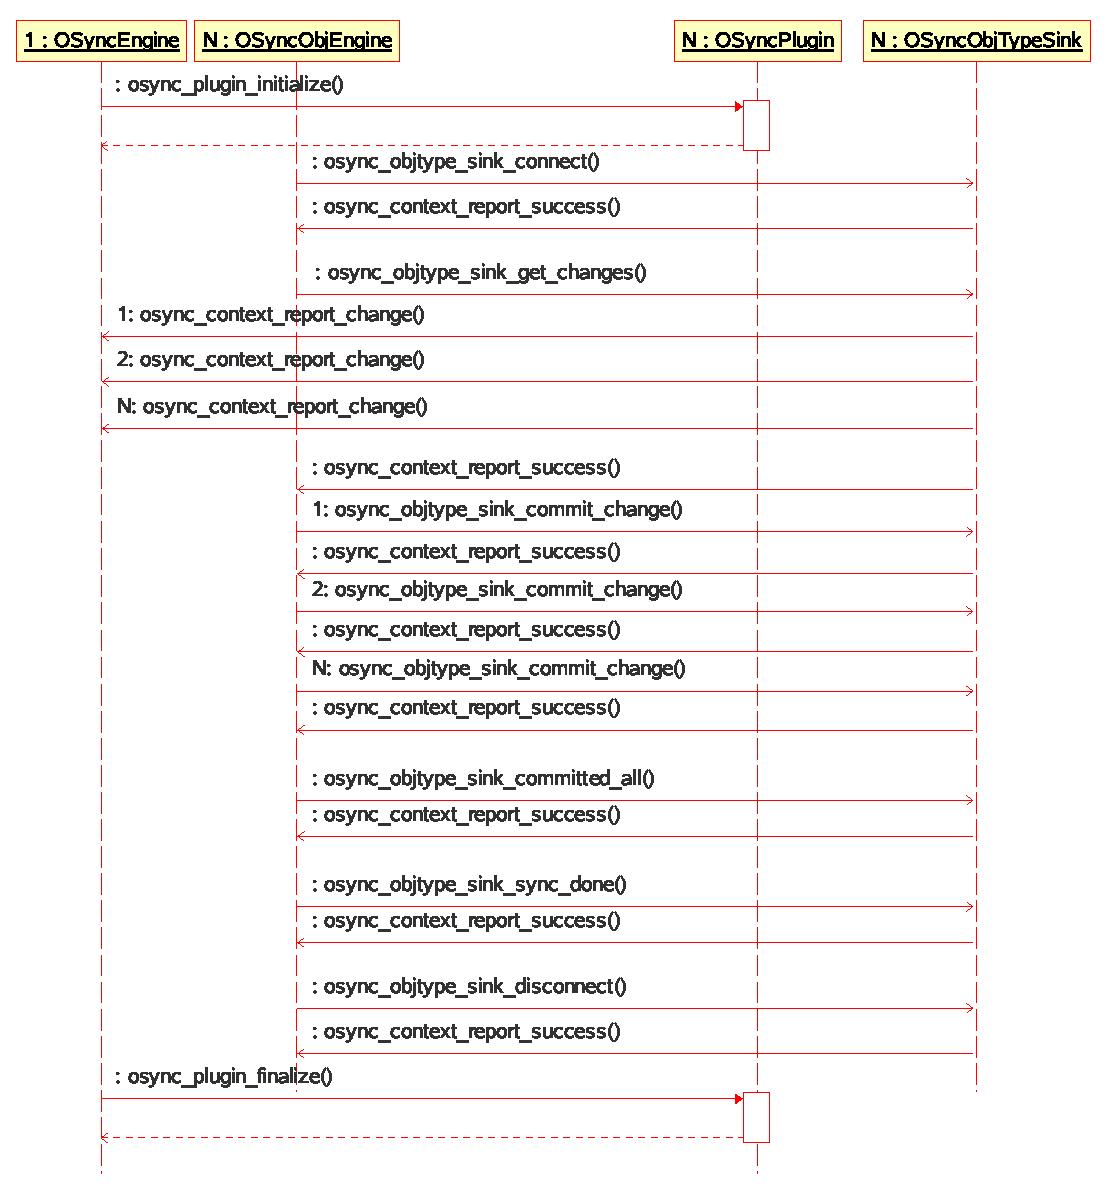
\includegraphics[bb=0 0 661 960, scale=0.60]{simple-sync-sequence}
 % simple-sync-sequence.png: 661x960 pixel, 72dpi, 23.32x33.87 cm, bb=0 0 661 960
 \caption{Plugin Synchronization Sequence}
 \label{fig:SimpleSyncSequence}
\end{figure}

Those function are called "Generic Functions" and MUST be implemented by 
plugin.

\section{Generic Functions}
The Generic Functions are the only functions, which got called synchronously by 
the OpenSync Framework.
\subsection{Initialization}
\subsection{Finalize}
\subsection{Discover}
%\subsection{Usable}
\section{Sink Functions}
All ">Sink Functions"< are called asynchronously, not like the "Generic
Functions", and have to reply with OSyncContext functions if the task was 
executed or not. It's very important that the ">Sink Functions"< reply the
request by the OpenSync Framework with the OSyncContext functions. Even on
error condition the Sink Function have to reply with a special OSyncContext
error function. Otherwise the OpenSync Framework until the timeout for this
function call is reached, which may take sometime for some usually time 
consuming functions\\
The Main Sink, which is Object Type neutral, doesn't have any required Sink 
Functions. For the Object Type Sink are the implementation of some Sink 
Functions required:

\begin{center}
% use packages: array
\begin{tabular}{ll}
\textbf{Function} & \textbf{Implementation} \\ 
Connect & O \\ 
Get Changes & M \\ 
Commit / Batch Commit & M (only Commit \textbf{or} Batch Commit) \\ 
Committed All & O (only available in combination with Commit)\\ 
Synchronization Done & O \\ 
Disconnect & O
\end{tabular}
\end{center}

The Plugin don't have to register a Main Sink if there is no need for Object 
Type neutral tasks.
\subsection{Connect}
The Connect function is available for all Object Type Sinks and could be used to
establish Object Type specific connection. If the connection establishment is an
Object Type neutral task (e.g. Bluetooth, USB, ...) and needded to be done only
once, only the Main Sink should be used. This avoids problems with shared access
to an interface, since a connect function would be called for each Object Type
for the same interface.\\
This function MUST only establish a connection to the device or ressource. After
the connection got established successful the plugin MUST reply the context with
\verb|osync_context_reply_success()|. On error the plugin replies a 
human-readable
(aka. userfriendly) error message with \verb|osync_context_reply_error()|.
\subsection{Get Changes}
The Get Changes function get called by the OpenSync Framework to request changes
since last synchronization or all entries of the Object Type specific ressource.
Later one MUST be done when a Slow Sync got requested by the OpenSync
Synchronization framework. If a Slow Sync got requested for this Sink MUST be
checked with \verb|osync_objtype_sink_get_slowsync()|. On a Slow Sync the 
Changetype (for all changes) is \verb|OSYNC_CHANGE_TYPE_ADDED|. On a regular 
(fast sync) synchronization it's up to the Get Changes function to determine 
the Changetype. Every change have to be reported with 
\verb|osync_context_report_change()|. On a error the Sink Function have to 
reply the context with \verb|osync_context_report_error()| and stop/leave this 
function ASAP. If the protocol, application or device isn't able to report 
changed entries since last sync, the OpenSync Helper Hashtable should be used 
to determine the Changetype of the entry.
\subsection{Commit}
This function get called with a single OSyncChange object, which MUST be
committed to the application or device. If the commit failed the context MUST be
replied with \verb|osync_context_report_error()|. On success the context get 
replied with \verb|osync_context_success()|. If Hashtable is already involved in
the Get Changes functions, then the Commit function has to update the entries 
for the Hashtable for entries which get committed.
\subsection{Batch Commit}
The batch commit function is intended for protocols, device or application which
only allow batch committing (sending all changes at once). This function get
called with an array of changes which have of be committed all at once.
\subsection{Committed All}
This function got called after all entries got committed, even if error appeared
while committing. This function get not called if Batch Commit function is
registered for this Sink.
\subsection{Synchronization Done}
This function got called only after a successful synchronization.
\subsection{Disconnect}
This function MUST only handle the disconnect of the sink. Don't do further
cleanup here, the finalize function is intended for releasing memory and
cleanup. The disconnect function might never get called when even the connect
function failed.
\section{Properties}
Each Synchronization Plugin has properties which get set within the
\verb|get_sync_info()| function. The properties are:

\begin{itemize}
\item Name, short name of the plugin should be less then 15 characters. This
name isn't visible to the user, at least not for rich OpenSync Frontends.
\item Longname, is the name of the plugin which is visible to the user in
rich OpenSync frontends. Should not be longer then 50 characters.
\item Description, about the Plugin visible to the end user in OpenSync
Frontends, and should additionally help to choose the right plugin.
\item Configuration Type, defines if the plugins needs any configuration or if
the configuration is optional or simply not needed.
\item Process Type, defines how the plugin get started: threaded, forked or by 
an external process.
\item Timeouts, for initialization, finalization and timeout can be configured
for the plugin needs. 
\end{itemize}

\subsection{Name}
The name of the plugin get defined like all plugin properties in
\verb|get_sync_info()| function with calling \verb|osync_plugin_set_name()|.
This name got used mostly for internal configuration and isn't visible to the 
user (at least not for rich OpenSync Frontend user). The name should be less
then 15 characters and should one word (no spaces). Example: ">palm-sync"<
\subsection{Longname}
The Longname of the plugin is the only name visible for  regular user to choose 
the correct plugin from a list of available plugins. Use the description field
to describe the plugin in more detail. Don't include the term ">Plugin"> in the
Longname. Example: ">Palm Device"<
\subsection{Description}
The description should additionaltly help the user to choose the correct plugin
if there are several plugins with similar names. Bad example: ">Plugin to sync 
your pda. Version 0.23. http://foo.edu/hacking/opensync"<. The term ">Plugin"< 
might confuse regular user, avoid it. If your plugin supports several different
devices don't list all known to work models, this might confuses people as well.
Again, don't list models! If your plugin is based on a synchronization 
implementation mention the name of protocol. No version numbers, no URLs and 
most user won't care about the authors name or E-Mail address.
\subsection{Plugin Timeouts}
The default plugin timeout should basically fit the need for all plugins. If
your plugin is known to be very slow you can change the timeout for this plugin
with following functions:
\begin{itemize}
\item \verb|osync_plugin_set_initliaze_timeout()|
\item \verb|osync_plugin_set_finalize_timeout()|
\item \verb|osync_plugin_set_discover_timeout()|
%\item \verb|osync_plugin_set_useable_timeout()|
\end{itemize}
The timeout unit is in seconds. It's possible to overwrite custom plugin timeout
with setting individual timeouts in the member configuration (syncmember.conf).
\subsection{Configuration Types}
If the plugin doesn't need any configuration by the user the plugin should the
configuration type to \verb|OSYNC_PLUGIN_NO_CONFIGURATION| with the
\verb|osync_plugin_set_config_type()| function. If the plugin don't need by
default a configuration but could be is additionally configurable the
configuration type should be set to \verb|OSYNC_PLUGIN_OPTIONAL_CONFIGURATION|. 
If the plugin can't perform without any configuration the type should be set
to\\ \verb|OSYNC_PLUGIN_NEEDS_CONFIGURATION| (set by default).
\subsection{Process Types}
The Process Type declares how a plugin get started. By default the plugin get
started by the OpenSync Framework within a thread (
\verb|OSYNC_START_TYPE_THREAD|). If the Plugin is known to conflict with the 
process mainloop of the OpenSync Framework, it's possible to run the plugin in 
a separated process by forking it. The forking is done by the OpenSync
Framework when the start type got set to \verb|OSYNC_START_TYPE_PROCESS|. If the
plugin has to access a not public interface to get access to the data ressources
of an application it's possible to integrate the plugin within this application.
So the plugin is running all the time this application is running and can
communicate with the OpenSync Framework when the Process Type got set to 
\verb|OSYNC_START_TYPE_EXTERNAL|. The Process Type can be changed with the 
\verb|osync_plugin_set_start_type()| function. 
\section{Configuration}


%Format Plugins
\chapter{Format Plugins}
\section{Converter}
\section{Detectors}




%Environments
\chapter{Environments}
\section{Plugin Environment}
\section{Format Environment}
\section{Group Environment}



%Credits
\input{credits.tex}

\appendix

%Exampes
\chapter{Examples}
\section{Plugin}
\section{Format Plugin}
\section{User Interface}


%GNU FDL
\input{fdl.tex}

\end{document}
